\section{Column Databases}\label{sec:column}

Key-value databases cannot organize many attributes, and document databases may lack features such as a SQL-like language. Column databases target a different need: very large volumes, heavy writes and analytics on few attributes.

\subsection{From rows to columns}
We distinguish two kinds of workload:
\begin{itemize}
  \item \g{OLTP} (Online Transaction Processing): many small ACID transactions, one record at a time.
  \item \g{OLAP} (Online Analytical Processing): interactive and fast analysis on many records, typical of Business Intelligence.
\end{itemize}
Row storage fits OLTP. In analytics we usually want \s{one attribute of many records}, but with rows we must read all the attributes. If the values of an attribute are stored together, we read only them.

\begin{example}[Sum of salaries]
For \texttt{SELECT SUM(salary) FROM salePersons}, with five records on five blocks, a row store scans all five blocks. A column store reads the single block containing the salaries.
\end{example}

\begin{center}
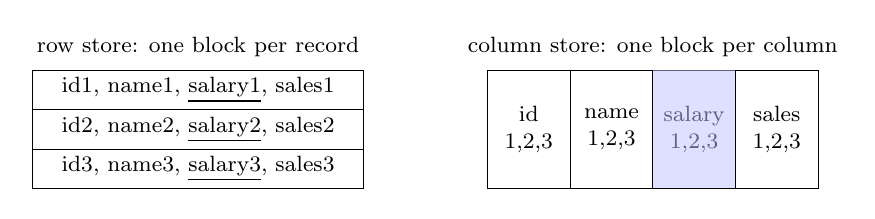
\begin{tikzpicture}[font=\footnotesize, x=1.05cm, y=0.5cm]
  \node at (2,3.6) {\s{row store}: one block per record};
  \foreach \y/\n in {2/1,1/2,0/3} {
    \draw (0,\y) rectangle (4,\y+1);
    \node at (2,\y+0.5) {id\n, name\n, \underline{salary\n}, sales\n};
  }
  \node at (7.5,3.6) {\s{column store}: one block per column};
  \foreach \x/\c in {5.5/id,6.5/name,7.5/salary,8.5/sales} {
    \draw (\x,0) rectangle (\x+1,3);
    \node[align=center] at (\x+0.5,1.5) {\c\\1,2,3};
  }
  \fill[blue!25, opacity=0.5] (7.5,0) rectangle (8.5,3);
\end{tikzpicture}
\end{center}

\paragraph{Compression.} Compression removes redundancy and works better on small groups of nearby similar values, so columns compress very well with low overhead. For example, in a sorted column we can store each value as a \g{delta} from the previous one, and repeated strings can be replaced by a dictionary (\texttt{Pisa}$\to$1, \texttt{Rome}$\to$2).

\paragraph{Single-row penalty.} Handling one row means accessing several blocks, so column databases perform poorly on single-row modifications. Caching and \s{multicolumn projections} (storing some columns together) partly reduce this cost.

\subsection{The wide-column data model}
\g{BigTable} (Google, 2006) introduced the model used by HBase and Cassandra: columns are dynamically controlled, rows are kept sorted, and reads and writes of a row are atomic. A value is identified by
\[
(\text{row key},\ \text{column name},\ \text{timestamp}).
\]

\begin{itemize}
  \item \g{Keyspace}: top-level container with tables, column families and the replication strategy and factor. Usually one per application.
  \item \g{Row key}: identifies a row and is used to partition and order data. The data of a row key is never split across different servers.
  \item \g{Column}: with row key and version stamp it identifies a value. Values are typed in Cassandra and untyped in BigTable.
  \item \g{Column family}: group of columns frequently used together, stored close on disk. Families are defined a priori, like tables, but the columns inside can be added dynamically, like key-value pairs.
\end{itemize}

So a column database is a \g{sparse multidimensional map}: rows can have different columns and missing cells take no space. In HBase a table is physically a collection of key-value cells:
\begin{lstlisting}
cust001 / address:street / t1 -> "178 Main St."
cust001 / address:city   / t1 -> "Boise"
cust003 / address:province / t1 -> "ON"
\end{lstlisting}

\subsection{HBase vs Cassandra}
\g{HBase} has a master-slave architecture on top of Hadoop:
\begin{itemize}
  \item \g{Region Servers} handle user requests. A \g{region} contains all the rows between two keys.
  \item \g{HMaster} assigns regions to region servers.
  \item \g{ZooKeeper} coordinates the nodes.
  \item \g{NameNode} keeps the metadata of the files in HDFS, and \g{DataNodes} store the blocks.
\end{itemize}

\g{Cassandra} is peer-to-peer: all nodes run the same software, even if they may serve different functions. It is simple, has no single point of failure, scales easily, and when a node is removed the servers with its replicas answer in its place.

\begin{center}\small
\begin{tabular}{p{3.2cm}p{5.4cm}p{5cm}}
\toprule
& \textbf{Cassandra} & \textbf{HBase} \\
\midrule
Architecture & masterless, peer-to-peer & master-slave on HDFS \\
Partition key & part of the primary key & row key \\
Partitioning & hash (typically Murmur3) & range on row key \\
Unit & partition & region \\
Ordering & clustering columns inside a partition & lexicographic on row key \\
Replication & configurable factor on the ring & storage layer (HDFS) \\
\bottomrule
\end{tabular}
\end{center}

\begin{lstlisting}[language=SQL]
CREATE TABLE orders (
  customer_id TEXT, order_ts TIMESTAMP, amount DOUBLE,
  PRIMARY KEY (customer_id, order_ts)  -- partition key, clustering column
);
\end{lstlisting}
All the orders of a customer are on the same node, sorted by time. In HBase, sequential row keys send all the writes to one server (\g{hot spot}), so we \s{hash} the row key or add a short random \s{prefix}.

\subsection{Internal mechanisms}
These mechanisms work together to balance performance, consistency and fault tolerance.

\paragraph{Commit log.} An append-only file. Each write is first stored here and then applied to its final location, so the database does not wait for the definitive write, and after a failure it recovers by replaying the log.

\paragraph{Bloom filter.} A probabilistic structure that avoids reading partitions which certainly do not contain a key. It answers \s{no} (always correct) or \s{maybe} (possible false positive).

\begin{definition}[Bloom filter]
An array of $n$ bits, initially 0, with $k \ll n$ hash functions. To \s{insert} a key we set the $k$ bits given by the hash functions. To \s{check} a key we compute the same positions: if at least one bit is 0 the key is certainly absent, otherwise it may be present.
\end{definition}

\begin{example}
With $n=10$, $k=3$, inserting \texttt{K101} with hashes $1,6,8$ sets those bits. \texttt{K105} with hashes $1,6,9$ is certainly absent, since bit 9 is 0. \texttt{K110} with hashes $6,8,1$ gets a \s{maybe} even if it was never inserted.
\end{example}

Both operations take constant time. Elements cannot be removed, because resetting a bit could create false negatives. With $h$ stored values, the usual choice is $n = O(h)$ and $k = \frac{n}{h}\ln 2$. False positives decrease as $n$ grows and increase as more elements are stored.

\paragraph{Consistency level and replication.} The level can be \g{strict} (all replicas), \g{low} (at least one replica) or \g{moderate} (in between), depending on the application. Usually a hash function selects the server of the first replica. In Cassandra further replicas go on the following nodes of the ring, clockwise.

\paragraph{Anti-entropy.} The process that detects differences between replicas while exchanging little data, using \g{hash trees}: each leaf is the hash of a subset of records and each internal node the hash of its children.
\begin{enumerate}
  \item One replica sends its root hash to the other. If the roots are equal, the replicas are equal.
  \item Otherwise, the hashes of the next level are compared, following only the branches that differ.
  \item Only the data of the differing leaves is exchanged.
\end{enumerate}
Hash collisions are extremely unlikely with SHA-256, but they would hide a difference, so they matter in critical applications.

\paragraph{Communication.} Nodes must know the status of the others.
\begin{itemize}
  \item \g{All-to-all}: $n(n-1)$ messages, it does not scale.
  \item \g{Centralized}: $2(n-1)$ messages through a leader, which is a single point of failure.
  \item \g{Gossip}: each node sends its information to a few random nodes, which forward it. It scales well, but information takes longer to reach everyone.
\end{itemize}

\paragraph{Read and write protocol, hinted handoff.} In Cassandra any node can receive a request and act as a proxy towards the right nodes. If the target of a write is down, the write would be lost, so a node starts a \g{hinted handoff}:
\begin{enumerate}
  \item it stores the write and its final destination;
  \item it periodically checks the status of the target;
  \item it sends the write when the target is available.
\end{enumerate}

\begin{remark}
The same idea (save the operation, retry later) is the recommended way to keep \s{different} databases aligned in the project, see \cref{sec:consistency-between-dbs}.
\end{remark}

\subsection{Design tips}
As always, queries guide the design. From them we extract:
\begin{itemize}
  \item \g{entities}: one row per instance, identified by the row key;
  \item \g{attributes}: columns;
  \item \g{query criteria}: how to organize tables, column families and partitions;
  \item \g{derived values}: additional columns for precomputed data (e.g.\ orders placed yesterday by a user).
\end{itemize}

\begin{example}[Typical queries]
\s{How many new orders were placed in the Northwest region yesterday?} needs only date, region and status. \s{When did a customer last order?} needs only customer ID and order date. Columns let us skip all the other attributes.
\end{example}

Main rules:
\begin{itemize}
  \item \g{Denormalize}, because there are no joins. For a many-to-many relation, each customer has one column per purchased product: the \s{column name} is the product ID and the \s{column value} can hold the product name, which avoids reading the product table. To go from product to customers, we add a family \texttt{Prod\_Cust} in the product table.
  \item \g{One entity in one row}: atomicity is usually guaranteed only at row level. A polymorphic \texttt{Product} becomes one table with four column families (common, appliance, book, clothing), and each row fills only the ones it needs.
  \item \g{Versions}: keep an appropriate number of versions, useful for rollback or trends. Old ones are removed during \g{compaction}.
  \item \g{Avoid complex values}: separate columns allow indexing and different families. Store a JSON in a column only if we just store and retrieve it as is.
\end{itemize}

\paragraph{Indexes.} \g{Primary indexes} are on row keys and are managed by the DBMS. \g{Secondary indexes} are on column values: if the DBMS manages them automatically, we should use them, and it will typically apply the most selective index first. They are not useful with very few distinct values, with too many distinct values, or with many missing values.

If we manage them manually, the index is a separate table from column value to row keys, which must be kept aligned in one of two ways:
\begin{itemize}
  \item \g{synchronous}: each write updates both tables, doubling the latency, with an always up-to-date index;
  \item \g{asynchronous}: a batch job updates the index, so writes are fast but the index can be stale for a while.
\end{itemize}

\paragraph{When to use them.} Very large volumes (hundreds of terabytes), frequent reads and writes, several data centers, tolerance of short-term inconsistency, dynamic fields and predictable access patterns. Typical uses are log and security analytics, scientific data, financial time series, web-scale services and social networks. As a reference, Cassandra on 330 Google VMs reached one million writes per second with a median latency of 10.3\,ms. If the data fits on a single server, avoid them.
